\documentclass[a4paper, 11pt]{article}


% -------------------- Packages essentiels --------------------
\usepackage[french]{babel}
\usepackage[T1]{fontenc}
\usepackage[hmargin=3cm, vmargin=3cm]{geometry}
\usepackage[utf8]{inputenc}
\usepackage[skip=2ex]{parskip}


% -------------------- Autres packages --------------------
\usepackage{amsmath}
\usepackage{biblatex}
\addbibresource{ch-sc.bib}
\usepackage{graphicx}
\graphicspath{{src/}}
\usepackage{hyperref}
\addto\extrasfrench%
{%
	\def\algorithmautorefname{\textsc{Alg.}}
	\def\equationautorefname{\textsc{Éq.}}
	\def\figureautorefname{\textsc{Fig.}}
	\def\lstlistingautorefname{\textsc{List.}}
	\def\sectionautorefname{\textsc{Sec.}}
	\def\subsectionautorefname{\textsc{Sec.}}
	\def\subsubsectionautorefname{\textsc{Sec.}}
	\def\tableautorefname{\textsc{Tab.}}
    \def\appendixautorefname{\textsc{Annexe}}%
}
\usepackage[version=4]{mhchem}
\usepackage{siunitx}
\DeclareSIUnit\angstrom{\text{Å}}


% -------------------- Propriétés du document --------------------
\title{Conception d'une structure type supercondensateur}
\author{H. Lou Chao}
\date{\today}


\begin{document}

% -------------------- Titre --------------------
\maketitle
\tableofcontents


% -------------------- Introduction --------------------
% Intérêt d'une telle structure, différentes méthodes de
% réalisation, méthode utilisée
\section*{Introduction}


% -------------------- Description du système --------------------
% Composition : les électrodes de graphite, l'électrolyte, 
% séparateur
% Structure : la distance entre les électrodes, la concentration 
% de l'électrolyte
\section{Description de la structure}

Un supercondensateur à double couche électrochimique, présenté \autoref{fig:schema_supercondensateur}, est constitué de deux électrodes séparées par une électrolyte et un séparateur (une membrane perméable). Dans le cadre de notre étude, ces électrodes sont modélisées par des plaques de graphite, l'électrolyte est une solution de soude, et la membrane perméable peut être ignorée.

\begin{figure}[bpht]
    \centering
    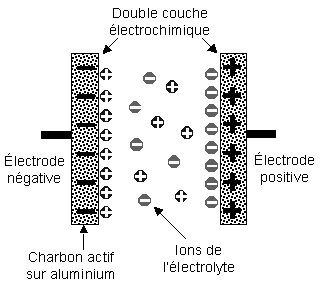
\includegraphics[scale=0.5]{schema_supercondensateur.png}
    \caption{Schéma d'un supercondensateur}
    % Par PNLL sur Wikipédia français — Transféré de fr.wikipedia à Commons., Domaine public, https://commons.wikimedia.org/w/index.php?curid=1713585
    \label{fig:schema_supercondensateur}
\end{figure}

Aussi, la distance séparant les électrodes capacitives est petite (de \qtyrange{3}{8}{\angstrom}), la conductivité de l'électrolyte est élevée (de l'ordre de \qtyrange{100}{1000}{\milli \siemens \per \centi \meter}), et la différence de potentiel entre les électrodes est relativement basse (de \qtyrange{2.1}{2.3}{\volt}).
% sigma_Na+ = 50.08, sigma_OH- = 198 mS/cm L/mol
% https://fr.wikipedia.org/wiki/Liste_de_conductivit%C3%A9s_molaires_ioniques
% https://fr.wikipedia.org/wiki/Conductivit%C3%A9_%C3%A9lectrique#Loi_de_Kohlrausch_et_concentration_molaire

Cependant, pour nous concentrer sur l'adsorption des ions et la répartition des charges sur les électrodes capacitives nous ne tentons pas de reproduire une structure réelle et construisons plutôt une structure modèle (\autoref{fig:structure_modele}) :
\begin{itemize}
    \item les électrodes capacitives sont séparées d'environ \qty{40}{\angstrom}
    \item l'électrolyte contient \num{20} ions hydroxyde et \num{20} ions sodium
    \item le voltage appliqué entre les électrodes est de \qty{4}{\volt}
\end{itemize}

\begin{figure}[htpb]
    \centering
    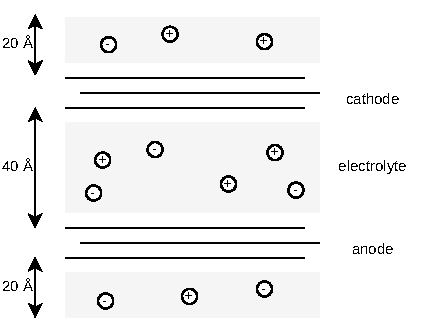
\includegraphics{ch-sc-structure_modele.pdf}
    \caption{Structure modèle construite pour cette étude}
    \label{fig:structure_modele}
\end{figure}


% -------------------- Construction du système --------------------
\section{Construction de la structure}

% -------------------- Méthode adoptée --------------------
% La démarche adoptée (fichiers initiaux, packmol, conversion en 
% données LAMMPS)
    \subsection{Méthode adoptée}

Pour la construction de la structure, la démarche \autoref{fig:demarche_construction} a été adoptée. Les fichiers initiaux ont été trouvés dans des bases de données comme les bases de données American Mineralogist Crystal Structure (AMCS), National Institute of Standards and Technology (NIST), etc., pour l'agencement des entités chimiques le package \emph{Packmol}\cite{martinez_packmol_2009} a été utilisé, et un script dédié à la conversion de la structure en données LAMMPS a été développé (voir \autoref{apdx:conversion}).

Avant de pouvoir lancer une simulation à partir de ce système, il est nécessaire de réaliser une minimisation de l'énergie et une relaxation du système.
% http://rruff.geo.arizona.edu/AMS/minerals/Graphite
% https://webbook.nist.gov/cgi/cbook.cgi?ID=C7732185

\begin{figure}[hbp]
    \centering
    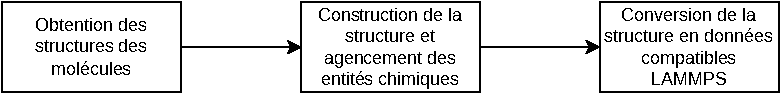
\includegraphics{ch-sc-construction.pdf}
    \caption{Démarche de construction du système}
    \label{fig:demarche_construction}
\end{figure}

% TODO: ajouter une capture du système


% -------------------- Méthode(s) alternative(s) --------------------
% Méthode 100 % LAMMPS, avantages--défauts, contraintes techniques
%     \subsection{Méthode alternative}

% Il est possible de construire notre structure avec une méthode alternative \qty{100}{\percent} LAMMPS. En effet, cet outil nous offre une certain nombre de commande pour créer, disposer, déplacer et supprimer des atomes ou molécules.

% La démarche adoptée, présentée \autoref{fig:methode_alternative}, consiste à créer une boîte de simulation remplie de molécules du solvant (en l'occurrence des molécules d'eau), puis d'y placer les ions pour obtenir l'électrolyte de notre système, et enfin de compléter le système avec les électrodes de graphite.

% \begin{figure}[tp]
%     \centering
%     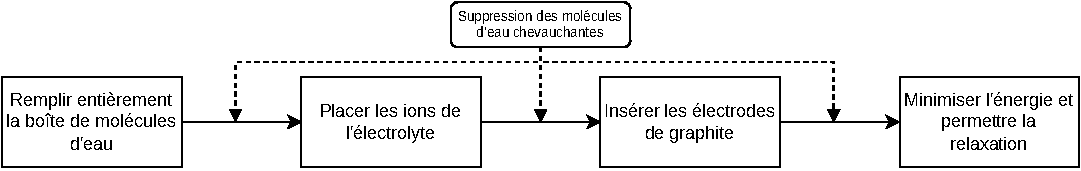
\includegraphics[width=\textwidth]{ch-sc-methode_alternative.pdf}
%     \caption{Démarche de construction du système avec LAMMPS}
%     \label{fig:methode_alternative}
% \end{figure}

% De plus, afin de s'assurer que les entités chimiques ne se superposent pas, il faut supprimer les molécules d'eau correspondantes à chaque étape d'insertion.

% Enfin, comme pour la méthode adoptée, il est nécessaire de réaliser une minimisation de l'énergie et une relaxation avant de pouvoir commencer une simulation.


% -------------------- Simulations obtenues --------------------
% Quelles simulations ont pu être réalisées
\section{Résultats obtenus}

Après l'obtention de la structure nous sommes en mesure de réaliser des simulations. Puisque la ligne directrice de notre étude est l'adsorption des ions, nous observons dans un premier temps l'adsorption des ions par des électrodes capacitives en graphite parfait. Nous étudions ensuite le comportement du système avec une cathode portant un défaut, dans notre cas ce défaut est un atome de carbone manquant.


% -------------------- Simulation d'électrodes parfaites --------------------
    \subsection{Simulation d'électrodes parfaites}


% -------------------- Simulation avec cathode défectueuse --------------------
    \subsection{Simulation avec cathode défectueuse}


\appendix
% -------------------- Annexe A : Conversion en données LAMMPS --------------------
% Objectifs, enjeux : convertir des fichiers de structure (xyz) en données LAMMPS
% Contraintes/facilités : structure des fichiers de données, facilités avec ReaxFF
% Réalisation : démarche/flux/algorithmes, langage choisi, packages/modules utilisés
\section{Conversion de fichiers de configuration en données compatibles LAMMPS} \label{apdx:conversion}


% -------------------- Annexe B : Construction 100 % LAMMPS --------------------
% Détails de l'input LAMMPS
% \section{Construction de la structure à l'aide de LAMMPS} \label{apdx:methode_alternative}


% -------------------- Références --------------------
\printbibliography

\end{document}